% ----------------------------------------------------------
\chapter{Desenvolvimento}
% ----------------------------------------------------------

\section{Análise Exploratória dos Dados}

\subsection{Seleção e Obtenção dos Dados}

A análise exploratória de dados (EDA), é parte primordial de qualquer projeto que envolva análise de dados, nesta etapa que é feita a observação das variáveis analisadas, entendimento de quais informações é possível extrair dos dados, e principalmente validar se os dados são adequados para aplicação no projeto que está sendo desenvolvido e ainda é possível identificar problemas nos dados, e a necessidade de realizar tratamentos para adequar os mesmos para serem utilizados. 

Conforme citado anteriormente a gestão do Sistema Cantareira é feita pela ANA e o DAEE, e a operação pela SABESP. Parte das ferramentas usadas nesse gerenciamento é a coleta de dados diários que informam parâmetros sobre a situação da operação dos reservatórios do SC. Esses dados são disponibilizados pela ANA e pela SABESP diariamente, e são de domínio público, o acesso da população a esses dados e a todos os relatórios que possam ser emitidos referente a regulação dos serviços de saneamento básico e segurança hídrica, incluindo a situação dos níveis dos reservatórios de água, é garantido pela XXXXXXXXXXX, sancionada pelo presidente Luiz Inácio Lula da Silva em novembro de 2024.

O Sistema Cantareira é composto por um conjunto de reservatórios, canais e tuneis conforme exposto anteriormente. O sistema é alimentado por vazões afluentes que enchem os reservatórios, e a água é transportada pelo sistema até encontrar a estação de tratamento e depois ser distribuída para RMSP. A Figura 1 a seguir apresenta um esquema geral do SC, com seus reservatórios e uma representação gráfica dos túneis por onde a água corre até chegar no destino final. Os dados fornecidos pela SABESP informam a situação nos níveis, vazões, precipitação e demais dados inerentes de cada reservatório individualmente, mas, também são apresentados dados gerais, que retratam o Sistema Equivalente Cantareira (SE), ou seja, o comportamento do sistema como um todo. E são esses dados que serão utilizados neste estudo. 

\begin{figure}[htb]
	\caption{\label{fig:Fig_1}Esquema geral do Sistema Cantareira.}
	\begin{center}
		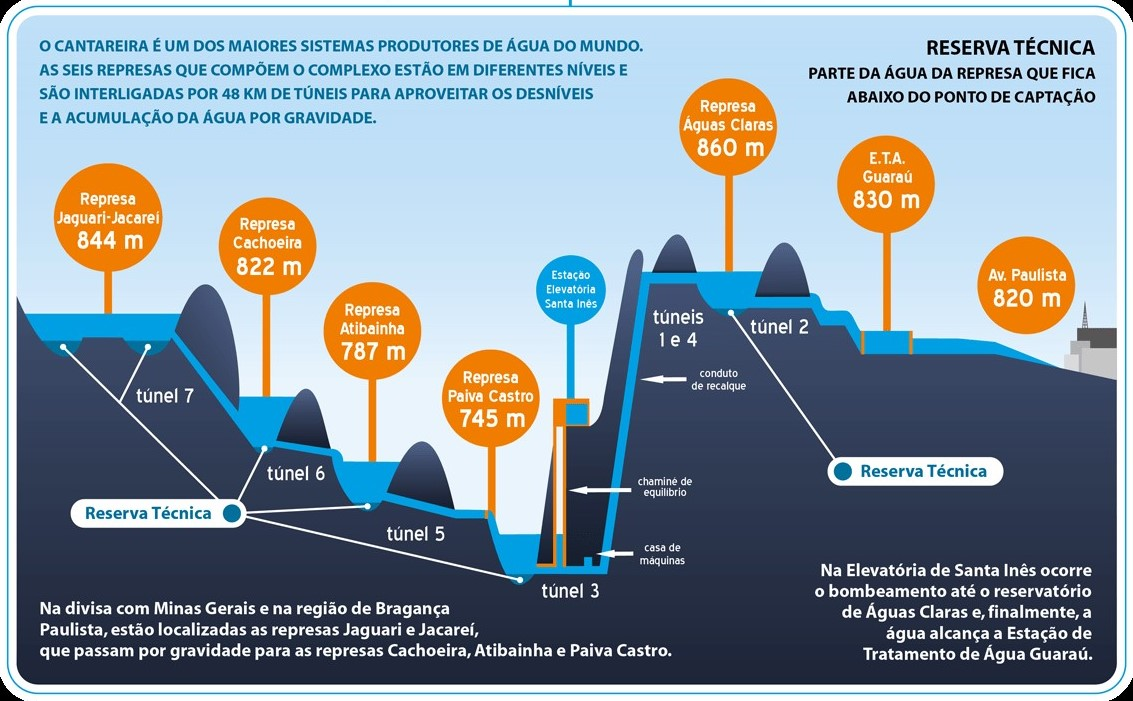
\includegraphics{figuras/sistema_cantareira.jpg}
	\end{center}
	\fonte{SABESP.}
\end{figure}

Há diversos dados disponíveis sobre o SE, para este trabalho foram selecionados alguns com base nos objetivos do estudo. A nossa variável alvo é o volume útil expresso em porcentagem, além desta, escolhemos analisar variáveis que entendemos ser possíveis influenciadoras do aumento ou diminuição do volume armazenado nos reservatórios, já que este estudo visa prever a disponibilidade de água no sistema. A Tabela 1 a seguir apresenta uma amostra do dataset construído a partir da coleta dos dados no site da SABESP para realização das análises preliminares. 

\begin{table}[htb]
    \ABNTEXfontereduzida
    \caption{Dataset de dados coletadosdo Sistema Cantareira.}
    \label{tab:exemplo_tabela}
    \begin{tabular}{@{}p{2.5cm}p{2.5cm}p{2.5cm}p{2.5cm}p{2.5cm}p{2.5cm}p{2.5cm}@{}}
    \toprule
    Data & Chuva (mm) & Volume Útil Armazenado (\%) & Volume Útil Armazenado (hm³) & Volume Total Armazenado (hm³) & Vazão Jusante (m³/s) & Vazão Natural (m³/s) \\ \midrule
    01/01/2000 & 30.9 & 47.11254 & 365.50555 & 1072.05098 & 10.16 & 70.885 \\
    02/01/2000 & 29.1 & 47.77519 & 370.64646 & 1077.1919 & 10.18 & 94.864 \\
    03/01/2000 & 35.175 & 48.59438 & 377.00187 & 1083.5473 & 7.29 & 108.208 \\
    04/01/2000 & 18.725 & 49.9968 & 387.88206 & 1094.42749 & 6.34 & 162.936 \\
    05/01/2000 & 25.9 & 51.94578 & 403.00251 & 1109.54794 & 6.33 & 211.604 \\
    \bottomrule
    \end{tabular}
    \fonte{\textcite{ibge2016}.}
    \end{table}